%%%%%%%%%%%%%%%%%%%%%%%%%%%%%%%%%%%%%%%%%%%%%%%%
\section{Method presentation}
\label{sec:3_Method}

%In this section, a detailed report of our mesh correspondence method is described. We provide an upper bound for the error at every step of reconstruction, the results are presented in the next section (\secref{sec:4_Validation}). 

%======================================
\subsection{Method overview}
\label{subsec:3_Method_overview}


We propose a correspondence method based on the deformation of templates, one for each bone, towards the database meshes. The original shapes are chosen among the database, then are modified in order to present convenient features, such as a balanced vertex count, respecting an equilibrium between lightness of calculation and precision of the data. We also work with uniform meshes, with homogeneous distribution of vertices and faces of the same size. The deformation is a composition of a first smooth detail preserving deformation, followed by a second registration to capture the sharp structures of the contours. A flowchart of the different steps is presented in \figref{im:3_flowchart}, the mesh notations used in the rest of the document are given in \figref{im:3_notations}. The steps leading to the final results are numbered from (1) to (7) as introduced in \figref{im:3_notations}.


We are interested in 14 bones of the wrist joint: the 8 carpal bones, the 5 metacarpals and the radius. We chose to leave the ulna bone out. This bone is indeed important in the elbow articulation and plays a critical role in the pronation-suppination movement of the forearm, but has a minor impact on the wrist articulation. It is however over present in the data due to its size: the number of vertices needed for a 3D mesh representation is more than the double of vertices required for one of the carpal bone. This overrepresentation affects the statistical models. For these reasons it was put aside, the radius alone is used as stable reference of the forearm. 


%% Image: Notations des meshes
\begin{figure}
	\centering
	\includegraphics[height=0.85\textheight]{\RootDir{img/notations.png}}
	\caption[Mesh notations]{Notation of the meshes generated at each step of the method. $b$ indicates the wrist bone, $i$ indicates the subject of the database the mesh represents.}
	\label{im:3_notations}
\end{figure}


%% Image: Flowchart
\begin{sidewaysfigure}
	\centering
	\includegraphics[width=0.9\textwidth]{\RootDir{img/flowchart.png}}
	\caption[Flowchart towards dense correspondence]{Flowchart of the different steps leading to dense correspondence between similarly shaped meshes.}
	\label{im:3_flowchart}
\end{sidewaysfigure}



%======================================
\subsection{Preprocessing}
\label{subsec:3_Method_preprocessing}


The initial input data we are working with are meshes of the \db*, direct outputs of a marching cube algorithm. The meshes \mo* are raw, composed of many vertices irregularly spread along the surface, connected by irregular triangles forming the faces, as illustrated in \figref{im:3_original_data}. The irregularity of the vertices distribution can skew the distance measures between meshes. Some meshes also exhibit artifacts originating from the segmentation step. These artifacts are coarse inaccuracies that need to be removed before analyzing the bone shapes. Finally the wrists have various locations and need to be aligned. The only treatment they have undergone is that left wrists have been mirrored, so they all are right wrists. For all these reasons, the raw data could not be used as is, and required an early processing step. 


%% Image: Maillage original irrégulier
\begin{figure}[!ht]
	\centering
	\includegraphics[width=0.5\textwidth]{\RootDir{img/maillage_original.png}}
	\caption[Initial input mesh]{Example of an initial input 3D mesh.}
	\label{im:3_original_data}
\end{figure}


\subsubsection{Post-segmentation processing (1)}
\label{ssubsec:post_segmentation}


The first treatment was to remove all artifacts of the data. There were different types of artifacts: one vertex that was obviously wrong compared to its neighbors, independent sets of points not attached to the bone surface that were floating inside the bones, different types of groups of vertices forming bulbs inside or outside the cortical surface. Some examples of defects can be seen in \figref{im:3_anomalies}. All these coarse errors indubitably originated from the original segmentation and had to be removed. The erroneous vertices were manually selected and eliminated. The gaps created by the deletion of some faces were closed by adding triangles between the remaining neighboring vertices. The resulting meshes are referred to as \mo*, $b$ indicates the bone represented by the mesh, $i$ specifies the subject.

%% Image: Anomalies dans les meshs CMC
\begin{figure}[!ht]
	\centering
	\includegraphics[width=\textwidth]{\RootDir{img/anomalies.png}}
	\caption[Anomalies in initial input meshes]{Example of anomalies present in the initial input 3D meshes.}
	\label{im:3_anomalies}
\end{figure}



\subsubsection{Resampling (2)}
\label{ssubsec:resampling}


When the bones have been cleared of inopportune coarse inaccuracies, the second process consisted in changing the points distribution on the surface. The same number of vertices is kept for each mesh, but they are regularly spread along the surface. Indeed the irregular distribution can skew the distances, due to conglomerates of points. The resampling method is based on Centroidal Voronoi Tessalation, and guarantees an homogeneous output surface, with a stable edge length \cite{alliez_2005_centroidal}. 

The procedure uses Voronoi diagrams, which define a partitioning of a surface into regions (cells) based on a set of seeds of that surface. One region is associated to every seed and consists of all surface points closer to that seed than to any other. In the case of a mesh, the seeds are its vertices, the Voronoi diagram is computed for the mesh surface. To move the vertices into an homogeneous distribution, the Lloyd's algorithm is used. Based on the Voronoi diagram of the mesh, the centers of mass of the cells, also called centroids, are computed. Each vertex is moved to the position of its associated region's centroid. The new Voronoi diagram is computed, as well as the new centroids, etc. These steps are iterated and converge to a centroidal Voronoi tesselation, which is a Voronoi diagram such as its seeds are also the centroids of its cells. These seeds are the positions of the new vertices. The Lloyd's algorithm can change the topology of the mesh, and allows a partitioning into triangles nearly equilateral.

The resulting meshes are the ones used for the rest of the work as the target database meshes. The homogeneous distribution of the vertices guarantees a more representative outcome. They are referred to as $M_{D\{b;i\}}$, $b$ is the bone index, $i$ is the subject index.



\subsubsection{Initial alignment of the wrists (3)}
\label{ssubsec:rough_ali}

Following the resampling step, the database bones \md* are characterized by uniform 3D meshes. Distances can be computed without being influenced by an uneven distribution of vertices across the surface. They are however not aligned yet. 

Alignment is in our case an absolute necessity. We have chosen to work with extrinsic characterization of the meshes, the vertices are described in $\mathbb{R}^3$, using external origin point and \soc*. Comparison between meshes described in such a way requires a previous rigid alignment of the bones: identical shapes can have considerably different representations due to isometric transformations. It leads to falsely high distances between structures, unless these shifts have been previously canceled. Isometric transformations designate translations, rotations and reflections, but only the two first ones are present between analogous bones in the database. We chose to get rid of scale differences too, by computing isotropic scaling. Size is the main parameter to bone shape differences between genders \cite{joshi_2016_registration-based}, we are more interested in shape disparities after normalization. 

We use an Iterative Closest Point (ICP) algorithm for a affine alignment of corresponding structures. However, tests demonstrated that the method does not converge to an accurate lining up of the bones unless the shapes are already coarsely aligned. 
We therefore propose a first step to roughly adjust the meshes. We define for each subject a new system of coordinates attached to the radius, characterized by radius features. The bone meshes are described in the new system, which approximately places the wrists in the same positions and orientations. 
We define this new \soc* as $(X_r, Y_r, Z_r)$ for every subject. %It was inspired by the radius coordinate system defined in \cite{coburn_2007_coordinate}.
In \cite{coburn_2007_coordinate}, they define a radial coordinate system such that the $X$ axis coincides with the radial long axis, the $Y$ axis is directed through the radial styloid and perpendicular to the $X$ axis. The $Z$ axis is simply the cross product of $X$ and $Y$. Our \soc* $(X_r, Y_r, Z_r)$ was inspired from the one described in \cite{coburn_2007_coordinate}. 


At first, the radius minimum oriented bounding box is computed. It designates the smallest rectangular cuboid within which all vertices of the object lie. The polyhedron orientation coincides with main orthogonal directions of variance of the item points. 


The $X_r$ axis is defined as the line parallel to the longest edges of the bone's bounding box, going through both centers of the faces perpendicular to these edges. This axis is a good approximation of the radial long axis. It is directed from the radial diaphysis (the middle tubular part of the bone, see \figref{im:2_rad_voc}) towards the carpal extremity. We denote $y$ the point at the extremity of the radial styloid process (see \figref{im:2_rad_voc}). It is the point whose perpendicular projection on the $X_r$ axis has the biggest coordinate. Its perpendicular projection on $X_r$ defines the center of the system. $Y_r$ is directed from the system center towards $y$. $Z_r$ is the cross-product of $X_r$ and $Y_r$. The unit length in all three directions is 1mm. The carpal bones expressed in this new system are coarsely aligned across the population. An illustration of such a system is visible in \figref{im:3_rad_coordsys}.


%% Image: Système de coordonnées du radius
\begin{figure}[!ht]
	\centering
	\includegraphics[width=0.8\textwidth]{\RootDir{img/rad_coordsys.png}}
	\caption{The radius-based coordinate system.}
	\label{im:3_rad_coordsys}
\end{figure}

When the meshes are described in this new bases, the radii are coarsely aligned, and so are the wrist bones, which have undergone the same transformations (rotation, translation). In this new basis the meshes are ready to be used, the affine ICP algorithm converges. 

The portion of the radius diaphyses visible on the CT scans is very variable across the population. To overcome these fluctuations, a last treatment is applied to the database radii: the radius shafts are cut on the proximal side, following the first alignment. They are carved along the plane perpendicular to the $X_r$ axis. The length kept along the $X_r$ axis is a constant proportion of the height (along $Y_r$) of the bone. The proportion was chosen to be the biggest possible, that is available for every subject. The resulting aligned and cut meshes are referred to as \ma*. %Two patients had such a small length of the diaphysis captured on the scans that they were removed from the database. 



%======================================
\subsection{Template set creation (4)}
\label{subsec:3_template_set_creation}

We chose to compute correspondence between shapes by deforming a template towards the database meshes. Templates are chosen among the subjects' bones, to ensure close shape similarity between the original and target meshes. They are also prepared in order to present convenient properties, such as a good balance for vertex density. 


\subsubsection{Template selection}
\label{ssubsec:teplate_selection}

The choice of the template is important, if its shape is too different from the ones it must adapt to, the results will be imprecise, miss details or else the deformations are so significant that it produces poor correspondence. Many iterations of registration and template updating might be a solution, but it would require a long time to get to a satisfying result. We start with templates already very close to the structures they are registered to. The best mean to have a close contour of the target shapes is to use database bones as templates. The registration of the bones is computed independently for each bone of a person, the template can also be selected independently. The selected meshes are then smoothed to remove sharp details specific to the individual bone. The templates should have desired mesh framework features, such as convenient edge density. Like in \cite{joshi_2016_registration-based}, we chose the templates among the database bones as the ones the closest to all other, they are the ones with the least specificity. 


A reference mesh is selected for each one of the $B = 14$ bones among the database individuals $I_\text{CMC}$. The reference mesh of the $b^{th}$ bone ($1 \leq b \leq B$) is chosen for being the one that is the most similar to the corresponding bones of the rest of the population. The choices are independent, selected bones may come from different subjects. The similarity of the $b^{th}$ bone of a person $j$ to the rest of the population is measured as follow: its mesh is aligned to the equivalent bone of all other subjects $i, i\neq j$, one after the other, using ICP.
Then the distance $d_\text{mean}(M_{D\{b,i\}}, M_{D\{b,j\}})$ between the rigidly aligned pair is computed using the mean distance (\ref{eq:mesh_dist}).
For each bone, its distances to all other equivalent bones are added up. The smallest sum across the subjects designates the reference mesh $M_{t \{b\}}$ for this bone.

\begin{equation}
	M_{t \{b\}} = \min_{j \in I_\text{CMC}} \sum_{i \in I_\text{CMC}, i \neq j} d_\text{mean}(M_{D\{b,i\}}, M_{D\{b,j\}})
	\label{eq:choice_template}
\end{equation}


We compute the rigid alignment with Iterative Closest Point (ICP) (\ref{sssubsection:existing_techniques}). To optimize the isotropic scaling simultaneously, we iterate between the optimization of the rigid transformations using ICP and the scaling. 

\subsubsection{Template creation}

To erase sharp details that are too specific to a given individual, the selected meshes are smoothed using five steps of Laplacian smoothing. A Laplacian smoothing consists in moving every vertex of the mesh towards the average location of its topological adjacent vertices. Applying this transformation five times shrinks slightly the shape, but mostly smooths sharp details.

We want to work with meshes that have a convenient edge density, which strikes a balance between detail precision and computing time. Therefore the smoothed meshes are resampled in order to get regular edge lengths of 1mm. The bones have various number of vertices, that are regularly distributed along the surface. It divides by 6 to 8 the number of vertices compared to the original meshes, highly speeding up computations. Tests have proven that no important loss of information is caused by this decreased number of points, compared to meshes with edges of $0.5$ or $0.3$mm, while the calculation time substantially decreases. In the end of the process, the corresponding bones will have the same number of vertices as the templates, and should also have a mean edge length of approximately 1mm, though by definition, points should not be exactly at the same distance from each other. The resulting templates that are used for the rest of the work are referred to as $M_{T \{b\}}$.



%======================================
\subsection{Dense correspondence mapping}
\label{subsec:3_Method_warping}


The templates having been selected, they are non-rigidly registered to define dense correspondence across the database. The deformed meshes should fit perfectly the individual shapes, preserving all details. With such a registration, dense correspondence between the population is natural, and can be used for various applications such as shape comparisons or else statistical shape studies. The deformation is computed in two steps, presented in this section. At first they are smoothly deformed using Laplacian Surface Edition \cite{sorkine_2004_laplacian}. These deformations are iteratively calculated, until an arbitrary precision is met and satisfactory visual results are obtained. This deformation meets its limits on sharp details representation. Therefore a second registration step is performed, which is a projection along the normals towards the target shape. 


\subsubsection{Affine registration (5)}
\label{sssec:rigid_registration}


The meshes encoding the database information are the original shapes that have been resampled once. They are referred to as \md*. The templates meshes, one for each bone, are referred to as \mt*. 
We aim at representing the database bones with the same set of vertices for each individual. This is achieved by deforming the templates, to fit the bones of the sample wrists. 

The very first step is to rigidly register the database bones \md* towards the templates \mt*, using affine ICP. This rigid registration converges thanks to the coarse alignment computed in \secref{ssubsec:rough_ali}. All remaining calculations are done with the aligned meshes \mr*. 


\subsubsection{Laplacian Surface Edition}
\label{ssubsec:3_laplacian_description}

The initial non-rigid deformation is computed using Sorkine et al. method called Laplacian Surface Edition presented in \cite{sorkine_2004_laplacian}. Based on an intrinsic surface representation, they introduce an approach that can be employed for various mesh editing operations such as free-form deformation, transfer of geometric details between surfaces, and so on. We are interested in this first application. Sorkine et al. argue that for local surface modeling, the surface representation should capture the intrinsic geometry of the surface, rather than the absolute position of points in Euclidean space. Therefore, they use an intrinsic encoding of the vertices, based on differential coordinates. Each vertex is described by the difference between its position and the centroid of its topological neighbors, which is known as Laplacian coordinates. They are a linear function of the global mesh geometry, the conversion between the intrinsic and absolute representations is efficient. 

Let $V = \{v_1, ..., v_n\}$ be the geometric positions of the $n$ vertices in $\mathbb{R}^3$. Let $N_i$ designates all topological neighbors of vertex $v_i$. Then, the Laplacian coordinate of $v_i$ is:

\begin{equation}
	L(v_i) = v_i - \frac{1}{|N_i|} \sum_{j \in N_i} v_j
\end{equation}

Modeling operations consist in computing the new coordinates $\{v_1',...,v_n'\}$ of the mesh vertices. It requires to fix the absolute positions of some vertices, such that $v_i' = u_i$ for $i \in \{m,...,n\}, m<n$. The constraints $\{u_i\}$ are satisfied in a least square sense. The new geometry $V'$ is solved by minimizing the error function: 

\begin{equation}
	E(V') = \sum_{i=1}^{n} || L(v_i) - L(v_i')||^2 + \sum_{i=m}^{n} || v_i' - u_i||^2
\end{equation}

Observing that Laplacian coordinates are only invariant to translation, the team modifies the latter error function, to make the coordinates additionally independent to rotation and isotropic scaling. They compute a transformation $T_i$ for each vertex $i$ based on the new configuration of vertices $V'$. The error function becomes: 

\begin{equation}
E(V') = \sum_{i=1}^{n} || T_i(V')L(v_i) - L(v_i')||^2 + \sum_{i=m}^{n} || v_i' - u_i||^2
\end{equation} 

$T_i$ is a transformation matrix that is limited to represent translations, rotations and isotropic scaling. It is derived for each vertex $v_i$ from the transformation of itself and its neighbors into $v_i'$ and its neighbors. 

\begin{equation}
	T_i = \min_{T} || Tv_i - v_i'||^2 + \sum_{j\in N_i} ||Tv_j-v_j'||^2
\end{equation}

$T_i$ is a linear function in $V'$. For further details, please refer to \cite{sorkine_2004_laplacian}.

Mesh edition can be computed through the definition of handles. These handles are define for a set of vertices, which can be moved by the user. Their new positions give the constraints $u_i$ from which the complete smooth deformation of the mesh is computed. 



\subsubsection{Non-rigid registration: Laplacian deformation (6)}
\label{ssubsec:laplacian}


Following the rigid registration, the second process performed is a smooth deformation of \mt* towards \mr* for all bones and all individuals. We use the Laplacian Surface Edition method. 
%It has the benefit of preserving geometric details of the surface while being deformed. 
The deformation uses handles defined for one vertex. They are moved towards target positions, dragging with it the nearby mesh surface in a smooth and detail preserving deformation. 


The distance between a point $p$ and a surface $S$ is defined as the shortest Euclidean distance between $p$ and any point of the surface (any point, not necessarily a vertex when the surface is depicted by a mesh). 
%The point of the surface for which the distance is the shortest is named $p_S$.

\begin{equation}
	d(p, S) = \inf_{p_S} || p-p_S||, \qquad   p_S \in S
\end{equation}


The non-rigid registration loops over two steps : choosing a handle, then deforming the bone surface.
For each vertex of \mr*, its distance to \mt*'s surface is computed. The vertex whose distance to the template is the greatest is named $v_R$. Its closest point on  \mt*'s surface is referred to as $p_T$. The handle is chosen to be $p_T$, and is moved to $v_R$'s location, deforming all neighboring region of the template. 

The stopping condition is a threshold on the maximal distance between a vertex of \mt* and its closest point on \mr*'s surface. A second condition was fixed on the number of iterations. The definition of the thresholds is discussed in the validation section (\secref{ssubsec:laplacian_validation}). The resulting meshes are referred to as $M_{l,\{b,i\}}$. 

Tests have proven that the algorithm requires an initialization, to ensure the quality of the results. Otherwise, falsely close points that are not anatomically correspondent may cause a bad convergence. The meshes having been previously rigidly registered, one vertex of the template is anchored to its own position, to avoid inopportune translation. Then, a few feature points are identified in both meshes, and aligned with each other. These points are automatically detected, and were defined based on trials. For instance, for the radius, the features chosen were 2 points at the proximal extremity of the radial tube, to ensure that the end of the visible diaphysis were in correspondence. The tip of the radial styloid process was selected to be another feature, as were two points on the distal radioulnar joint, see \figref{im:3_rad_ftrpts_def}. The identification of such points was based on geometrical criterions, enabled by the coarse pre-alignment of the wrists. All these points are in turn used as handles for a first rough deformation. Then the vertex previously anchored to its own position is unanchored. There was indeed no reason that it was well aligned with the target mesh, and inopportune translations are not a risk anymore when a few other features have been defined. 

%% Fig: Exemple de points d'initialisation de l'algorithme Laplacien 
\begin{figure}[!ht]
	\centering
	\includegraphics[width=0.8\textwidth]{\RootDir{img/feature_pts.png}}
	\caption{Example of the features points used to initialize the radius smooth deformation algorithm.}
	\label{im:3_rad_ftrpts_def}
\end{figure}

When all bones \mr* have been approximated by the deformed templates $M_{l,\{b,i\}}$, the templates \mt* are updated. The new templates vertices are defined as the geometrical mean of the deformed templates instances, the framework remains always the same. The registration of the templates to the database meshes and the update of the templates steps are repeated several times, generating at each repetition a new set of $M_{l,\{b,i\}}$. It is used to reduce the effect of the choice of the initial template meshes. The final meshes are called \ml*. The number of iterations is discussed in the validation section \secref{ssubsec:laplacian_validation}.



\subsubsection{Non-rigid registration: projection along the normals (7)}
\label{ssubsec:projection}

The Laplacian-based deformation is smooth and meets its limits as for capturing the sharp details of the database. Therefore a second registration is used to completely fit the deformed templates \ml* already similar to the target bones to the database target meshes \mr*. The points of the \ml* meshes are simply projected along their normals to the hit point with the subjects bones \mr*'s surface. This second registration step guarantees that every vertex is on the surface of the actual bone. The already great similarity between the shapes before this step ensures that the points are already close from their final position, keeping a coherent and regular distribution over the subjects, while best describing their particularities. To completely ensure that a point will not be sent to an absurd location around very sharp details, a maximal distance between the original and the final positions is defined. If the distance to the hit point is higher than this threshold, the point is moved to the mean position of its neighboring vertices. 

Projection along normals could be considered as the only non-rigid registration step, and the Laplacian deformation would be skipped. Each point of the deformed template would be on the target's surface, point-to-face distances from the template to the target would be zero. However, depending on the initial shape differences and on the normal orientations, sharp details of the target surface can easily be missed. Additionally crossing normal directions could cause crossing edges, flipped faces, the mesh surface would delineate degenerated volumes. %Finally, nothing guarantees that the vertices distribution would still be approximately homogeneous after such a projection, when the shapes can be quite different. 
And since the distances are symmetrical, the errors can be very high. For all these reasons, both non-rigid registration step are necessary.

%\todol{Wang, 2004, shaoe correspondence through landmark ... Ils utilisent aussi de la projection}

The resulting meshes are the final meshes used in later applications such as statistical models, and are referred to as \mw*. 



\subsection{Results}

In this section, we have started with a raw database of 3D polygonal meshes, results of manual segmentation and marching cube mesh generation. These meshes presented coarse irregularities that were removed. They also were resampled, in order to have a homogeneous distribution of vertices over its surface. The new resulting meshes are named \md*.

Comparison of 3D shapes requires some relations defined between these shapes. We use dense one-to-one correspondence between the meshes by describing all instances of a class of bones using the same landmarks. Each vertex is considered a landmark, even though it is not necessarily positioned in a significant place of the bones. The bone $b$ of every subject is characterized by the same number of vertices, the $j^{th}$ vertex is at the same location of the bone on all instances. Therefore the correspondence between bones ensues from such a description, all $j^{th}$ vertices are in relation together. 

In order to obtain such a characterization of the bones, we have chosen to work with template meshes that are being registered to fit the database bones. The registration is a two-steps process: first the templates are being iteratively non-rigidly deformed towards the target shapes. Secondly, when the templates are close to the targets, their vertices are projected towards the aimed surfaces. 

The resulting meshes \mw* are believed to characterize the same shapes as the target ones \mr*, while their vertices are used as landmarks for a class of bone and fitted to represent the same place on each instance surface. The first property is verified in the next section. The second is harder to validate and will be considered in the next chapter. If the properties are verified, shapes diversity can be studied, by comparison of the vertices location, for example using a statistical shape model. 

The process stages have aligned and scaled the bones regardless of their initial position in the wrist. However this information is preserved and the meshes can be brought back precisely to their initial location at the end of operations. It is essential for the handling of poses data. 